\newpage
\subsection{Naked Single}
\label{Naked_Single}
Bei der Technik \textit{Naked Single} werden Kandidatenlisten verwendet. Diese Technik kann angewendet werden, wenn in der Kandidatenliste einer Zelle nur noch ein Kandidat steht. Dieser Kandidat kann dann in die Zelle eingetragen werden. Das funktioniert aufgrund des Aufbaus der Kandidatenlisten. Diese enthalten zuerst alle Kandidaten und es werden immer dann Kandidaten entfernt, wenn dieser Kandidat nicht mehr als Ziffer in der Zelle stehen könnte wel er dort eine Regel verletzen würde. Wenn also nur noch ein Kandidat in der Kandidatenliste steht, dann bedeutet das, dass dieser Kandidat die einzige Ziffer zwischen 1 und 9 ist, die in der Zelle stehen kann ohne eine Regel zu verletzen.

\begin{figure}[h]
\begin{center}
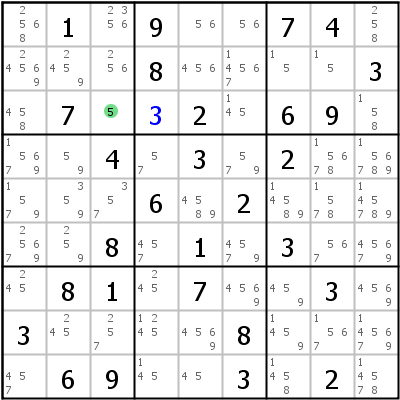
\includegraphics{./img/naked_single.png}
\caption{Naked Single}
\end{center}
\end{figure}

Im oben stehenden Beispiel \textbf{Abbildung 3.2} sieht man sofort, dass die Kandidatenliste in z3s3 nur noch einen Eintrag enthält. Dieser kann nun einfach eingetragen werden.